\chapter{Trường chuẩn, các thang tương tác và các dòng yếu mang điện}

Điện động lực học lượng tử và sắc động lực học lượng tử trông rất khác nhau trong phòng thí nghiệm, nhưng cả hai đều là các lý thuyết chuẩn. Thực ra, gần như mọi tương tác trong Mô hình Chuẩn đều được tổ chức theo cách này. Từ \emph{gauge} mang một ý nghĩa sâu hơn liên quan đến đối xứng địa phương, nhưng ta có thể tạm hoãn bộ máy đó lại. Hiện tại ta cần một mô tả vật lý tối thiểu: một lý thuyết chuẩn chứa các trường kiểu Maxwell, các nguồn được bảo toàn, các phép biến đổi đối xứng, các boson chuẩn, và các quy tắc phát xạ và hấp thụ những boson đó.

\section{Lý thuyết Maxwell như nguyên mẫu}

\subsection{Trường và thế}

Trường điện từ có sáu thành phần: ba thành phần của điện trường và ba thành phần của từ trường. Cùng thông tin đó có thể được mã hóa, với một phần dư thừa, trong một thế bốn-vectơ
\begin{equation}
A_\mu=(A_0,\boldsymbol A),
\end{equation}
trong đó \(A_0\) là thế tĩnh điện và \(\boldsymbol A\) là thế vectơ không gian. Trong giới hạn tĩnh điện, điện trường được suy ra từ gradient không gian,
\begin{equation}
\boldsymbol E=-\boldsymbol\nabla A_0,
\qquad
\boldsymbol F=q\boldsymbol E,
\end{equation}
trong khi từ trường là
\begin{equation}
\boldsymbol B=\boldsymbol\nabla\times\boldsymbol A.
\end{equation}
Dấu trong phương trình thứ nhất phụ thuộc vào định nghĩa chuẩn của thế; phần thảo luận trên bảng chủ yếu quan tâm đến thực tế rằng các trường là các đạo hàm của thế.
\editorialnote{Đối với các trường phụ thuộc thời gian, hệ thức đầy đủ là
\(\boldsymbol E=-\boldsymbol\nabla A_0-\partial_t\boldsymbol A\). Bài giảng cố ý làm việc ở mức tĩnh điện đơn giản hơn tại đây.}

\begin{figure}[htbp]
\centering
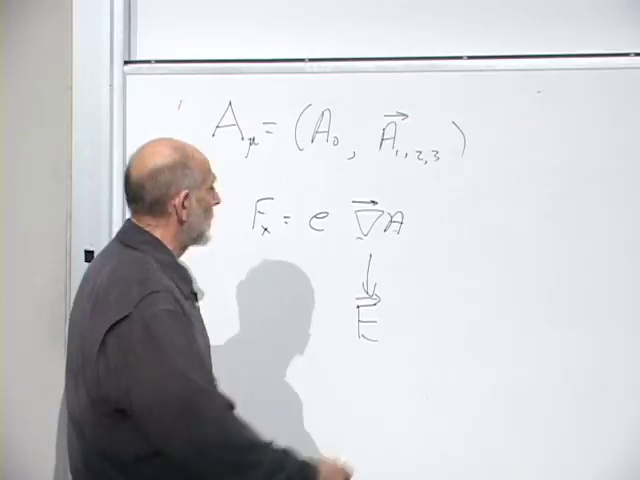
\includegraphics[width=0.62\textwidth]{lecture_05_figure_02.png}
\caption{Thế bốn điện từ và quan hệ đạo hàm của nó với trường.}
\lectureframe{00:03:33}
\end{figure}

Vì vậy điện động lực học chấp nhận hai mô tả tương đương: một theo \(\boldsymbol E\) và \(\boldsymbol B\), và một theo \(A_\mu\). Mô tả sau chỉ có bốn thành phần được viết ra vì những thế khác nhau có thể mô tả cùng một trường vật lý. Sự dư thừa đó là gợi ý đầu tiên ẩn sau từ gauge, dù ta chưa dùng nó một cách hình thức.

\subsection{Sóng và phân cực}

Các phương trình Maxwell cho phép các nghiệm sóng. Xét một sóng phẳng truyền theo một vectơ đơn vị \(\hat{\boldsymbol k}\). Tại mọi điểm, điện trường và từ trường đều là ngang:
\begin{equation}
\boldsymbol E\cdot\hat{\boldsymbol k}=0,
\qquad
\boldsymbol B\cdot\hat{\boldsymbol k}=0,
\qquad
\boldsymbol E\cdot\boldsymbol B=0.
\end{equation}
Trong các đơn vị với \(c=1\), độ lớn của chúng bằng nhau,
\begin{equation}
|\boldsymbol E|=|\boldsymbol B|.
\end{equation}
Đối với một sóng phân cực thẳng, hướng của \(\boldsymbol E\) xác định phân cực. Toàn bộ hình mẫu truyền đi với tốc độ ánh sáng.

Lượng tử hóa làm thay đổi ngôn ngữ nhưng không làm thay đổi cấu trúc phân cực. Một lượng tử của sóng điện từ là một photon. Việc vẽ photon như một điểm tất nhiên là dễ gây hiểu nhầm, nhưng vẫn hữu ích nếu hình dung rằng điểm đó mang một kim chỉ nhỏ theo phương ngang ghi lại phân cực của nó. Một tấm một phần tư bước sóng hoặc một phần tử quang học khác có thể làm quay phân cực đó. Tương tự, một trường Coulomb tĩnh cũng có thể được hình dung, dù chỉ rất gần đúng, như phát sinh từ sự phát xạ và hấp thụ lặp đi lặp lại của các photon.

\subsection{Nguồn, thông lượng và bảo toàn}

Sóng điện từ có thể lan truyền qua không gian rỗng, nhưng trường còn có các nguồn: điện tích và dòng điện. Một điện tích điểm dương tạo ra một điện trường xuyên tâm hướng ra ngoài tỉ lệ với \(1/r^2\). Số đường sức xuyên qua bất kỳ mặt cầu nào bao quanh điện tích là độc lập với bán kính của mặt cầu. Về mặt toán học,
\begin{equation}
\oint_{S^2}\boldsymbol E\cdot d\boldsymbol S
=\frac{Q_{\mathrm{enc}}}{\epsilon_0},
\label{eq:l5-gauss}
\end{equation}
trong hệ đơn vị SI.

Đây không chỉ là một cách thuận tiện để tính trường. Các đường sức điện chỉ có thể kết thúc trên điện tích. Nếu một điện tích cô lập đơn giản biến mất, thì trường của nó sẽ phải biến mất ở khắp nơi cùng lúc, vi phạm tính nhân quả, hoặc một mặt trước của phần trường bị thiếu sẽ phải lan truyền ra ngoài với các đường sức kết thúc trên không gian rỗng. Cả hai khả năng đều không được phép. Vì thế, hình học của thông lượng làm cho bảo toàn điện tích trở nên tự nhiên: điện tích có thể chuyển động, và các điện tích trái dấu có thể hủy nhau, nhưng điện tích thuần không thể biến mất cục bộ nếu không có một dòng bù.

Phát biểu cục bộ tương ứng là phương trình liên tục
\begin{equation}
\partial_t\rho+\boldsymbol\nabla\cdot\boldsymbol J=0.
\label{eq:l5-continuity}
\end{equation}
\editorialnote{Phương trình~\eqref{eq:l5-continuity} là dạng toán học cục bộ chuẩn của lập luận thông lượng nhân quả đã được triển khai bằng lời trong bài giảng.}

\subsection{Một định nghĩa làm việc về lý thuyết chuẩn}

Giờ đây ta có thể phát biểu mẫu hình thao tác. Một lý thuyết chuẩn có:
\begin{itemize}
\item các trường kiểu điện và kiểu từ;
\item các sóng mà, khi tương tác đủ yếu, trông giống sóng ánh sáng;
\item các nguồn tương tự điện tích;
\item một định luật Gauss gắn thông lượng với các nguồn đó;
\item một định luật bảo toàn và một đối xứng đi kèm;
\item các lượng tử của trường, được gọi là boson chuẩn; và
\item một hằng số liên kết chi phối sự phát xạ và hấp thụ.
\end{itemize}
Nguồn không nhất thiết phải là điện tích. Như một ví dụ cố ý phi vật lý, hãy tưởng tượng chuẩn hóa số baryon. Proton và neutron đều có số baryon \(+1\), nên chúng sẽ đẩy nhau thông qua một lực mới kiểu Coulomb; một proton và một phản proton sẽ hút nhau. Một lý thuyết như vậy có thể hình dung được về mặt toán học, nhưng tự nhiên không cung cấp trường chuẩn tầm xa quan sát được nào ghép với số baryon. Bảo toàn tự nó không bảo đảm có một lực chuẩn.

Điện tích điện quả thật đi kèm với một đối xứng. Đối với một trường vật chất mang điện,
\begin{equation}
\psi(x)\longmapsto e^{i\theta}\psi(x).
\label{eq:l5-u1}
\end{equation}
Đối xứng pha và bảo toàn điện tích là hai mặt của cùng một cấu trúc. Về sau ta có thể làm cho \(\theta\) phụ thuộc vào không-thời gian và thấy vì sao thế \(A_\mu\) là cần thiết. Ở đây phép biến đổi toàn cục là đủ để xác định điện tích được bảo toàn.

\section{QCD như ví dụ không Abel}

\subsection{Bộ ba, phản bộ ba và ma trận gluon}

Trong sắc động lực học lượng tử, một trường quark mang một chỉ số màu \(i\in\{r,g,b\}\) và biến đổi theo biểu diễn cơ bản của \(SU(3)\):
\begin{equation}
q'_i=U_{ij}q_j,
\qquad
U^\dagger U=\boldsymbol 1,
\qquad
\det U=1.
\label{eq:l5-q-transform}
\end{equation}
Đây là một phép quay trong không gian màu phức ba chiều, không phải một phép quay của không gian vị trí thông thường. Biểu diễn ba thành phần này cũng được gọi là biểu diễn định nghĩa.

Các trường phản hạt được biểu diễn bởi các biến liên hợp phức. Lấy liên hợp phức của Phương trình~\eqref{eq:l5-q-transform} cho ta
\begin{equation}
q_i^{\prime *}=U_{ij}^*q_j^*.
\label{eq:l5-antiquark-transform}
\end{equation}
Vì vậy quark biến đổi như \(\boldsymbol 3\), còn phản quark biến đổi như \(\bar{\boldsymbol 3}\).

\begin{figure}[htbp]
\centering
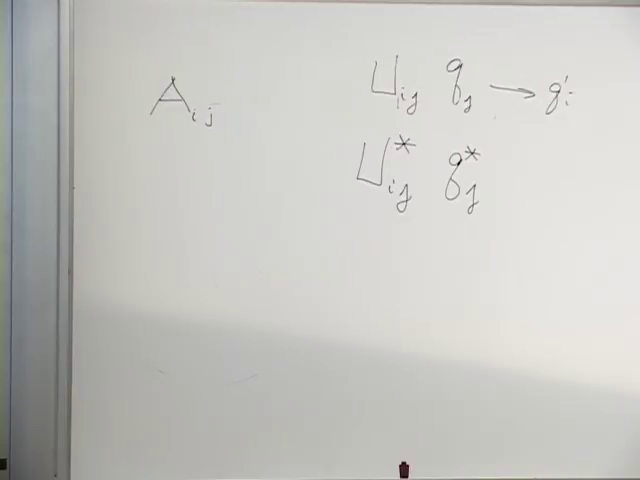
\includegraphics[width=0.62\textwidth]{lecture_05_figure_03.png}
\caption{Phép biến đổi cơ bản và phép biến đổi phản bộ ba liên hợp phức của nó.}
\lectureframe{00:18:47}
\end{figure}

\begin{classroomqa}
\audiencequestion{Có bao nhiêu ma trận \(U\) -- 7, 8 hay 9?
\lecturetimestamp{00:19:37}}
\lecturerresponse{Có vô hạn phần tử nhóm \(U\). Số hữu hạn đang được đếm là số các phần sinh độc lập, và với \(SU(3)\) thì số đó là 8. Một ma trận \(3\times3\) tổng quát có 9 ô ma trận, nhưng điều kiện unita đặc biệt chỉ để lại 8 hướng liên tục.}
\end{classroomqa}

Trường gluon có thể được viết thành một ma trận không vết \(A_{ij}\). Một chỉ số biến đổi như một quark và chỉ số kia như một phản quark, nên cấu trúc màu của nó là
\begin{equation}
\boldsymbol 3\otimes\bar{\boldsymbol 3}
=\boldsymbol 1\oplus\boldsymbol 8.
\end{equation}
QCD giữ lại bát tử không vết,
\begin{equation}
A_{ii}=\operatorname{tr}A=0,
\end{equation}
và loại bỏ đơn tử. Đó là lý do QCD có 8 gluon thay vì 9. Tổng quát hơn, \(SU(N)\) có
\begin{equation}
N^2-1
\end{equation}
phần sinh và cũng có từng ấy trường boson chuẩn.

Photon là trung hòa đối với \(U(1)\) điện: việc quay pha của một electron không biến photon thành một photon khác. Gluon thì khác. Một gluon mang một màu và một phản màu, nên nó biến đổi theo biểu diễn adjoint. Chẳng hạn, một tổ hợp đỏ--phản lam không phải là một đơn tử màu dù nó chứa một màu và một phản màu.

\subsection{Dòng chỉ số và tự tương tác}

Có thể đọc ra quy tắc tương tác bằng cách lần theo các chỉ số. Về mặt sơ đồ, một quark có màu \(i\) có thể trở thành một quark có màu \(j\) đồng thời phát ra một gluon mang dòng màu tương ứng:
\begin{equation}
q_i\longrightarrow q_j+A_{ij}.
\label{eq:l5-quark-gluon-vertex}
\end{equation}
Vị trí chính xác của \(i\) và \(j\) phụ thuộc vào quy ước mũi tên; nội dung bất biến là mọi chỉ số đi vào một đỉnh phải tiếp tục dọc theo một đường khác. Không có chỉ số màu nào bị mất.

Quy tắc này áp dụng trong mọi lý thuyết chuẩn \(SU(N)\). Vật chất cơ bản có một chỉ số, vật chất phản cơ bản có một chỉ số liên hợp, và một boson chuẩn có một chỉ số mỗi loại. Tên gọi vật lý có thể thay đổi, nhưng cấu trúc chỉ số thì giữ nguyên.

Bởi vì bản thân một gluon mang màu, nó có thể phát ra một gluon khác. Một gluon \(A_{ij}\) có thể tách qua một chỉ số trung gian \(k\), về mặt sơ đồ,
\begin{equation}
A_{ij}\longrightarrow A_{ik}+A_{kj}.
\label{eq:l5-three-gluon-index}
\end{equation}
Đây không phải là một đỉnh Yang--Mills hoàn chỉnh, nhưng nó biểu diễn dòng màu. Trong điện động lực học thông thường không có điều gì tương tự xảy ra với photon. Vì thế gluon tác dụng lực lên gluon, và động lực học của trường không Abel phức tạp hơn nhiều so với lý thuyết tuyến tính của Maxwell.

Một hệ quả định tính là giam hãm. Các đường thông lượng màu không thể kết thúc, và tự tương tác của chúng kéo chúng thành một ống nối một quark với một phản quark. Ống này mang một năng lượng gần như không đổi trên một đơn vị chiều dài:
\begin{equation}
V(R)\simeq \sigma R.
\end{equation}
Vì vậy, kéo hai đầu mút ra xa hơn sẽ tích trữ nhiều năng lượng hơn thay vì giải phóng màu cô lập. Đây là hình ảnh cục keo dẻo quánh: chính trường ngăn các thành phần mang màu thoát ra như các hạt tự do.

\section{Các hằng số liên kết và ý nghĩa của mạnh hay yếu}

\subsection{Điện tích như một biên độ phát xạ}

Một lý thuyết chuẩn vẫn cần một hằng số liên kết. Trong QED, điện tích electron \(e\) là hệ số gắn với một đỉnh electron--photon. Nó là một biên độ, còn xác suất là bình phương của các biên độ. Về mặt thao tác, hãy hình dung chặn đột ngột một electron nhanh trong một ống tia catôt. Xác suất phát ra một photon tỉ lệ với \(e^2\), với các hệ số quy ước được hấp thụ vào hằng số cấu trúc tinh tế,
\begin{equation}
\alpha=\frac{e^2}{4\pi\hbar c}
\simeq \frac{1}{137}.
\label{eq:l5-alpha}
\end{equation}
Trong các đơn vị tự nhiên \(\hbar=c=1\), hằng số liên kết là không thứ nguyên. Một mức cỡ 1 phần trăm cho một phát xạ sơ cấp làm cho điện từ học là yếu theo nghĩa nhiễu loạn: đa số electron bị dừng lại không phóng ra một chùm photon cứng.

\subsection{Đơn vị tự nhiên liên hệ năng lượng, thời gian và khoảng cách}

Đặt
\begin{equation}
c=1,
\qquad
\hbar=1.
\end{equation}
Khi đó thời gian và khoảng cách có cùng đơn vị, còn năng lượng có đơn vị nghịch đảo:
\begin{equation}
E=\hbar\omega\longrightarrow E=\omega\sim\frac1t,
\qquad
x\sim t\sim\frac1E.
\end{equation}
Năng lượng lớn thăm dò các khoảng cách ngắn và các thời gian ngắn.

Để định hướng,
\begin{equation}
1\ {\rm eV}^{-1}
=\frac{\hbar c}{1\ {\rm eV}}
\simeq 1.97\times10^{-7}\ {\rm m}.
\end{equation}
Vì vậy, một độ dài nguyên tử cỡ \(10^{-10}\ {\rm m}\) tương ứng xấp xỉ với một kiloelectronvolt nghịch đảo. Đây là các chuyển đổi bậc độ lớn, không phải quang phổ chính xác.

\subsection{Sự phân cấp bên trong một nguyên tử}

Đối với một nguyên tử điển hình, lấy
\begin{equation}
R_{\rm atom}\sim10^{-10}\ {\rm m}.
\end{equation}
Ánh sáng đi qua khoảng cách này trong
\begin{equation}
t_{\rm transit}^{\rm atom}\sim10^{-18}\ {\rm s}.
\end{equation}
Tuy nhiên, trong một nguyên tử nhẹ, electron chỉ chuyển động với một phần nhỏ của tốc độ ánh sáng. Trong bức tranh Bohr, \(v/c\sim\alpha\), nên một thời gian quỹ đạo điển hình dài hơn:
\begin{equation}
t_{\rm orbit}^{\rm atom}\sim10^{-16}\ {\rm s}.
\end{equation}

Một nguyên tử kích thích còn mất lâu hơn nữa để phát xạ:
\begin{equation}
t_{\rm decay}^{\rm atom}\sim10^{-9}\ {\rm s}
\end{equation}
như một ước lượng thô ở quy mô bài giảng. Có hai sự ức chế trong bức tranh vật lý. Lực điện từ chỉ tạo ra gia tốc vừa phải, và một electron đang gia tốc lại có thêm một xác suất phát xạ nhỏ khác do \(\alpha\) chi phối. Vì vậy hằng số cấu trúc tinh tế nhỏ tạo ra một sự phân cấp giữa các thời gian truyền qua, quỹ đạo và phân rã bức xạ.

\subsection{Sự vắng mặt của phân cấp trong một hadron}

Một hadron là một hệ liên kết kiểu nguyên tử được tạo bởi quark và gluon, nhưng thang kích thước của nó nhỏ hơn nhiều:
\begin{equation}
R_{\rm hadron}\sim10^{-15}\ {\rm m},
\qquad
t_{\rm transit}^{\rm hadron}\sim10^{-23}\ {\rm s}.
\end{equation}
Các quark đi ngang qua hadron trên về cơ bản cùng một thang thời gian, và các hadron kích thích phân rã mạnh cũng sống xấp xỉ
\begin{equation}
t_{\rm orbit}^{\rm hadron}
\sim t_{\rm decay}^{\rm hadron}
\sim10^{-23}\ {\rm s}.
\end{equation}
Một hadron bị va chạm có thể dao động và phát ra một pion gần như nhanh như tính nhân quả cho phép. Không có sự tách biệt 7 hoặc 9 bậc độ lớn như bên trong một nguyên tử.

\begin{classroomqa}
\audiencequestion{Thuyết tương đối hẹp có hàm ý rằng một hadron không thể phân rã nhanh hơn đáng kể so với thời gian ánh sáng đi ngang qua nó không?
\lecturetimestamp{00:47:15}}
\lecturerresponse{Đó là một cách hợp lý để phát biểu cận bậc độ lớn. Các phân rã mạnh xảy ra gần nhanh bằng mức mà kích thước của hệ cho phép; không có hằng số liên kết nhỏ hay sự ức chế lớn nào khác làm chậm chúng lại.}
\end{classroomqa}

Vì thế, hằng số ghép mạnh tương ứng lớn hơn \(\alpha\) rất nhiều. Ở một thang hadron dùng để minh họa, bài giảng nêu
\begin{equation}
\alpha_{\rm QCD}\sim0.2,
\end{equation}
gần với 1 hơn nhiều so với \(1/137\). Đây là nguồn gốc động lực học của tên gọi cũ \emph{các tương tác mạnh}.
\editorialnote{Hằng số ghép QCD chạy theo năng lượng, nên \(\alpha_s\) không phải là một con số cố định duy nhất. Giá trị được nêu ra là một giá trị minh họa phụ thuộc thang, đúng như chủ ý của bài giảng.}

\begin{classroomqa}
\audiencequestion{Bên tương tự của tương tác mạnh có được gọi đơn giản là hằng số lực mạnh không?
\lecturetimestamp{00:48:17}}
\lecturerresponse{Theo quy ước, nó được gọi là \(\alpha_{\rm QCD}\), hoặc thường hơn là \(\alpha_s\). Hằng số điện từ thường chỉ được gọi là \(\alpha\), mặc dù \(\alpha_{\rm QED}\) có thể được dùng khi cả hai cùng xuất hiện trong một cuộc thảo luận.}
\end{classroomqa}

\begin{classroomqa}
\audiencequestion{Trong một bài báo, người ta có phân biệt độ ghép điện từ trần với giá trị đo được, đã bị che chắn không?
\lecturetimestamp{00:48:38}}
\lecturerresponse{Có. Người ta nói về một độ ghép trần và một độ ghép tái chuẩn hóa. Phân cực chân không làm cho độ ghép hiệu dụng phụ thuộc vào thang mà tại đó nó được đo.}
\end{classroomqa}

\section{Điều bí ẩn của phân rã yếu}

Tương tác yếu được đặt tên từ thời gian phân rã rất dài của chúng. Chúng thường chậm hơn các phân rã mạnh và thậm chí có thể chậm hơn bức xạ nguyên tử. Ví dụ lâu đời nhất là phân rã beta hạt nhân.

\subsection{Phân rã beta của neutron}

Một neutron tự do phân rã theo
\begin{equation}
n\longrightarrow p+e^-+\bar\nu_e.
\label{eq:l5-neutron-decay-intro}
\end{equation}
Bài giảng dùng thời gian sống xấp xỉ 12 phút, dài đến khó tin so với \(10^{-23}\ {\rm s}\). Các giá trị chính xác hiện đại không quan trọng đối với lập luận này.

Một phần của sự chậm này là do động học. Xấp xỉ,
\begin{equation}
\begin{aligned}
m_n&\simeq940\ {\rm MeV},
&
m_p&\simeq939\ {\rm MeV},
\\
m_e&\simeq0.5\ {\rm MeV}.
\end{aligned}
\end{equation}
Chỉ một phần rất nhỏ năng lượng nghỉ của neutron khả dụng dưới dạng động năng. Nếu neutron nhẹ hơn tổng các khối lượng nghỉ cuối, phân rã sẽ là bất khả. Nếu nó chỉ nằm cao hơn ngưỡng một lượng vô cùng nhỏ, không gian pha khả dụng sẽ rất nhỏ và phân rã sẽ chậm. Nhưng chỉ riêng không gian pha không thể giải thích một thời gian sống được đo bằng phút.

\subsection{Pion tích điện loại bỏ lời biện hộ bằng ngưỡng}

Hãy xét thêm
\begin{equation}
\pi^-\longrightarrow e^-+\bar\nu_e
\end{equation}
và quá trình liên hợp điện tích của nó. Pion có năng lượng dư dả trên ngưỡng của kênh electron, vậy mà thời gian sống yếu của nó vẫn ở bậc nanôgiây chứ không phải bậc hadron \(10^{-23}\) giây. Một kênh tương tự với muon sẽ sớm trở nên quan trọng. Vì thế, điều bí ẩn là nội tại của tương tác yếu, chứ không chỉ là một hệ quả ngẫu nhiên của việc các khối lượng của neutron gần như suy biến.

\editorialnote{Thời gian sống của pion tích điện vào khoảng \(26\ {\rm ns}\), và kênh trội là \(\pi^-\to\mu^-\bar\nu_\mu\). Kênh electron bị ức chế helicity. Bài giảng trước hết dùng kênh electron vì việc theo dõi các hạt trong đó là đơn giản nhất, rồi quay lại kênh muon trội.}

Thuật ngữ phân rã beta có nguồn gốc lịch sử từ cách gọi các electron phát ra là tia beta. Các ví dụ pion và neutron liên quan đến cùng một tương tác dòng tích điện, dù động học của chúng khác nhau rất mạnh.

\section{Bảng các quark và lepton}

\subsection{Màu tác động theo chiều dọc}

Hãy sắp xếp sáu hương quark thành ba cột ghép cặp,
\begin{equation}
(u,d),\qquad(c,s),\qquad(t,b),
\end{equation}
và đặt một bản sao đỏ, lục và lam của mỗi quark vào các hàng riêng. Đối xứng màu \(SU(3)\) tác động theo chiều dọc: nó quay các phiên bản đỏ, lục và lam của quark up vào nhau, và đồng thời thực hiện cùng phép quay màu ấy trên down, charm, strange, top và bottom. Nó không biến một quark up thành một quark down.

\subsection{Isospin yếu tác động theo chiều ngang}

Đối xứng yếu tác động theo hướng kia. Nó trộn từng cặp lân cận
\begin{equation}
Q_1=\begin{pmatrix}u\\d\end{pmatrix},
\qquad
Q_2=\begin{pmatrix}c\\s\end{pmatrix},
\qquad
Q_3=\begin{pmatrix}t\\b\end{pmatrix}.
\label{eq:l5-quark-doublets}
\end{equation}
Các quark kiểu up có điện tích \(+2/3\), còn các quark kiểu down có điện tích \(-1/3\), nên điện tích thay đổi một đơn vị qua mỗi cặp.
\editorialnote{Nguồn tư liệu thoáng chốc nói rằng quark down có điện tích \(-2/3\). Phép trừ ở đoạn lân cận và mọi quá trình tiếp theo đều đòi hỏi giá trị chuẩn \(-1/3\), và ở đây dùng giá trị ấy.}

Vì đối xứng này tác động trên các doublet, nhóm tự nhiên là \(SU(2)\). Nó tác động lên mọi bản sao màu của mỗi doublet quark mà không làm đổi màu.

Còn có một hàng hạt thứ tư không mang điện tích màu và vì thế không tương tác với gluon: các lepton. Chúng tạo thành thêm ba doublet,
\begin{equation}
L_e=\begin{pmatrix}\nu_e\\e^-\end{pmatrix},
\qquad
L_\mu=\begin{pmatrix}\nu_\mu\\\mu^-\end{pmatrix},
\qquad
L_\tau=\begin{pmatrix}\nu_\tau\\\tau^-\end{pmatrix}.
\label{eq:l5-lepton-doublets}
\end{equation}
Các neutrino trung hòa điện; electron, muon và tau có điện tích \(-1\). Một lần nữa, hai thành viên khác nhau đúng một đơn vị điện tích. Electron, muon và tau có cùng các số lượng tử gauge nhưng khối lượng khác nhau, cũng như ba thế hệ quark kiểu up hay kiểu down lặp lại cùng một mẫu điện tích.

\begin{figure}[htbp]
\centering
\includegraphics[width=0.82\textwidth]{lecture_05_figure_05.png}
\caption{Bảng trên bảng đen: màu tác động giữa các hàng đỏ, lam và lục, còn \(SU(2)\) yếu nối các cột hương ghép đôi và hàng lepton.}
\lectureframe{01:03:35}
\end{figure}

Việc gọi lepton là màu thứ tư ở giai đoạn này chỉ là một phép loại suy. Chúng tạo thành hàng thứ tư trong bảng doublet yếu, nhưng \(SU(3)\) QCD thông thường không quay quark thành lepton.

\section{Xây dựng các boson yếu mang điện}

\subsection{Các số lượng tử của các boson mang điện}

Các boson gauge mang những tính chất biến đổi cần thiết để chuyển từ một thành viên của doublet sang thành viên kia. Hãy bắt đầu với cặp lepton
\(e^-\bar\nu_e\). Nó có điện tích \(-1\), nên boson gauge mang điện tương ứng được gọi là \(W^-\):
\begin{equation}
W^-\sim e^-\bar\nu_e.
\end{equation}
Cùng các số lượng tử ấy cũng xuất hiện từ một quark down và một phản quark up:
\begin{equation}
W^-\sim d\bar u.
\end{equation}
Ký hiệu \(\sim\) có nghĩa là có cùng các số lượng tử gauge liên quan như. Nó không có nghĩa rằng \(W\) theo nghĩa đen là một trạng thái liên kết của các hạt này. Phản hạt có các tổ hợp liên hợp,
\begin{equation}
W^+\sim e^+\nu_e\sim\bar d u.
\end{equation}

Các đỉnh yếu mang điện bao gồm
\begin{align}
e^-&\longrightarrow\nu_e+W^-,
&
\mu^-&\longrightarrow\nu_\mu+W^-,
\label{eq:l5-lepton-w}\\
d&\longrightarrow u+W^-,
&
s&\longrightarrow c+W^-,
\label{eq:l5-quark-w}
\end{align}
cùng với các chuyển tiếp tương tự cho thế hệ thứ ba khi được phép về mặt động học. Boson gauge thực hiện về mặt động lực cùng sự trộn theo chiều ngang mà đối xứng thực hiện trên doublet.

\begin{classroomqa}
\audiencequestion{Bảo toàn điện tích buộc boson phát ra phải có điện tích \(-1\), nhưng tại sao các chuyển tiếp của electron, quark down và quark strange đều phải liên quan đến cùng một hạt?
\lecturetimestamp{01:12:56}}
\lecturerresponse{Đó là một sự kiện thực nghiệm được mã hóa trong đối xứng yếu chung. Tự nhiên hoàn toàn có thể một cách nhất quán đã gán một boson kiểu \(W\) khác nhau cho mỗi họ, hoặc riêng cho quark và lepton. Thay vào đó, một \(SU(2)\) duy nhất tác động đồng thời lên mọi doublet, và cùng các boson gauge mang điện ấy làm trung gian cho mọi chuyển tiếp này.}
\end{classroomqa}

\subsection{Đọc và đảo một đỉnh}

Một đỉnh đơn lẻ biểu diễn cả một họ quá trình. Đảo một đường đi vào thành một đường đi ra sẽ biến một hạt thành phản hạt của nó, và đảo một đường \(W^-\) sẽ cho một \(W^+\). Vì thế, ta có thể đọc một đỉnh như sự phát xạ, hấp thụ, phân rã, hủy cặp, hoặc phản ứng nghịch, miễn là điện tích, động lượng và mọi số lượng tử liên quan đều được theo đúng một cách nhất quán.

\begin{classroomqa}
\audiencequestion{Các mũi tên và các đường trong những đỉnh yếu này có thể bị đảo được không?
\lecturetimestamp{01:14:51}}
\lecturerresponse{Có. Một đường có thể được chuyển từ trạng thái cuối sang trạng thái đầu hoặc ngược lại, nhưng khi đó một hạt sẽ trở thành phản hạt của nó. Do đó cùng một đỉnh cục bộ mô tả nhiều phản ứng với định hướng khác nhau.}
\end{classroomqa}

\begin{classroomqa}
\audiencequestion{Việc viết một \(W^-\) với các đường strange và charm có nghĩa là boson ấy theo nghĩa đen là một quark strange liên kết với một phản quark charm không?
\lecturetimestamp{01:15:43}}
\lecturerresponse{Không. Việc theo dõi các đường chỉ nói rằng \(W^-\) mang sự thay đổi số lượng tử giữa các cột ấy. Nếu giản đồ được đọc như một phân rã, một \(W^-\) đủ năng lượng có thể tạo ra một quark strange và một phản quark charm; nó không được cấu tạo từ chúng.}
\end{classroomqa}

\begin{classroomqa}
\audiencequestion{Một electron và một phản neutrino có thể tạo ra một \(W\), rồi hạt đó sinh ra một cặp quark không?
\lecturetimestamp{01:17:22}}
\lecturerresponse{Chính xác. Nếu có đủ năng lượng trong hệ quy chiếu khối tâm, các lepton ban đầu có thể tạo thành trạng thái trung gian dòng tích điện, và trạng thái ấy có thể đi ra qua một kênh quark được phép. Hai đỉnh đó chính là những đỉnh dùng trong phân rã, chỉ được đọc theo một định hướng khác.}
\end{classroomqa}

\subsection{Boson thứ ba còn thiếu}

Một nhóm \(SU(2)\) có ba bộ sinh, nên có ba trường gauge. Cho đến nay ta mới chỉ hiển thị \(W^+\) và \(W^-\). Một trường thứ ba, trung hòa điện, phải gắn với những tổ hợp đường chéo như các số lượng tử electron--positron và neutrino--phản neutrino. Nó được cố ý để lại lẩn khuất trong nền. Quan hệ của nó với boson vật lý \(Z\) và photon đòi hỏi sự trộn điện-yếu, điều này sẽ đến sau.

\begin{classroomqa}
\audiencequestion{Lực yếu và lực mạnh đã được nghi ngờ ở những thời điểm lịch sử khác nhau sao?
\lecturetimestamp{01:24:11}}
\lecturerresponse{Các gốc rễ thực nghiệm của chúng xuất hiện cùng nhau trong giai đoạn đầu của hiện tượng phóng xạ. Phân rã alpha hé lộ vật lý hạt nhân và tương tác mạnh, phân rã beta hé lộ tương tác yếu, còn phân rã gamma phát ra các photon điện từ. Ngay từ thời Becquerel đã có đủ cả ba đầu mối, rất lâu trước khi các lý thuyết trường hiện đại của chúng tồn tại.}
\end{classroomqa}

\section{Các ví dụ đã giải về phân rã dòng tích điện}

\subsection{Phân rã pion}

Pion mang điện âm có thành phần quark hóa trị
\begin{equation}
\pi^-=d\bar u.
\end{equation}
Các số lượng tử ấy có thể hủy thành một \(W^-\), rồi hạt đó có thể sinh ra một lepton mang điện và phản neutrino tương ứng:
\begin{align}
\pi^-&\longrightarrow W^{-*}
\longrightarrow e^-+\bar\nu_e,
\label{eq:l5-pion-electron}\\
\pi^-&\longrightarrow W^{-*}
\longrightarrow \mu^-+\bar\nu_\mu.
\label{eq:l5-pion-muon}
\end{align}
Dấu sao nhắc ta rằng \(W\) trung gian là ảo. Kênh thứ hai là kênh trội.

\begin{figure}[htbp]
\centering
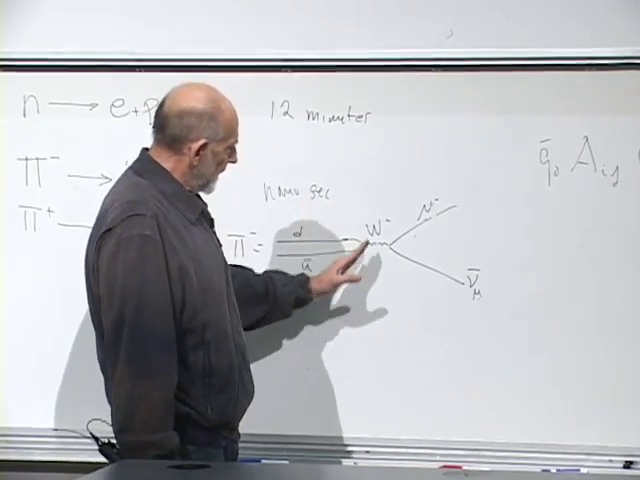
\includegraphics[width=0.72\textwidth]{lecture_05_figure_04.png}
\caption{Một pion \(d\bar u\) hủy thành một \(W^-\) ảo, rồi thành một lepton mang điện và phản neutrino tương ứng của nó.}
\lectureframe{01:19:38}
\end{figure}

\begin{classroomqa}
\audiencequestion{Đây có thực sự là một giản đồ Feynman không, mặc dù chiều thời gian được vẽ theo phương ngang chứ không phải phương thẳng đứng?
\lecturetimestamp{01:20:21}}
\lecturerresponse{Có. Hướng của thời gian trên trang là một quy ước. Một khi một hướng đã được tuyên bố là thời gian và mọi mũi tên đều được diễn giải nhất quán, hình vẽ mang cùng thông tin tương tác.}
\end{classroomqa}

\begin{classroomqa}
\audiencequestion{Có thể hiểu sơ đồ này giống một phản ứng hóa học thuận nghịch hơn là một sự phân rã một chiều không thể đảo ngược không?
\lecturetimestamp{01:21:35}}
\lecturerresponse{Quá trình ngược lại là được phép. Một pion được tạo ra trong không gian trống sẽ phân rã vì các hạt ở đầu ra tách xa nhau và thông thường không tái hợp. Nhưng nếu một muon và một phản neutrino được bắn cùng nhau với năng lượng và động lượng thích hợp, thì có một biên độ khác không để tạo thành pion thông qua tương tác ngược.}
\end{classroomqa}

\subsection{Năng lượng và trạng thái trung gian ảo}

Đối với một pion đứng yên,
\begin{equation}
m_\pi\simeq140\ {\rm MeV},
\qquad
m_\mu\simeq106\ {\rm MeV},
\qquad
m_\nu\approx0
\end{equation}
ở độ chính xác liên quan ở đây. Năng lượng còn lại trở thành động năng của các hạt đi ra. Bảo toàn động lượng đòi hỏi
\begin{equation}
\boldsymbol p_\mu+\boldsymbol p_{\bar\nu}=0,
\end{equation}
nên hai hạt bay ra ngược chiều nhau trong hệ quy chiếu nghỉ của pion.

\begin{classroomqa}
\audiencequestion{Làm sao năng lượng có thể được bảo toàn khi \(W\) trung gian nặng hơn pion rất nhiều?
\lecturetimestamp{01:25:08}}
\lecturerresponse{Chỉ các hạt đầu và cuối mới phải nằm trên vỏ khối lượng của chúng. Bốn-động lượng được bảo toàn tại mọi đỉnh, nhưng một đường nội ảo không cần thỏa mãn \(E^2=\boldsymbol p^2+m_W^2\). Độ lệch off-shell của nó càng lớn thì propagator của nó càng ức chế quá trình mạnh hơn.\editorialnote{Bài giảng dùng ngôn ngữ truyền thống của nguyên lý bất định năng lượng--thời gian và nói rằng trạng thái trung gian có thể vi phạm năng lượng trong thời gian ngắn. Phát biểu hiện đại chính xác là phát biểu trong phần trả lời: năng lượng-động lượng được bảo toàn, còn một đường nội ảo không nhất thiết phải thỏa mãn điều kiện vỏ khối lượng của hạt thực.}}
\end{classroomqa}

\subsection{Phân rã muon}

Một muon trước hết có thể biến thành neutrino của chính nó bằng cách phát ra một \(W^-\) ảo:
\begin{equation}
\mu^-\longrightarrow\nu_\mu+W^{-*}.
\end{equation}
Boson ảo đó sau đó sinh ra một electron và một phản neutrino electron:
\begin{equation}
\mu^-\longrightarrow
\nu_\mu+e^-+\bar\nu_e.
\label{eq:l5-muon-decay}
\end{equation}
Đây là một quá trình thuần lepton. Muon nặng hơn electron khoảng hai trăm lần, nên các khối lượng nghỉ cuối vẫn để lại nhiều động năng.

\begin{figure}[htbp]
\centering
\includegraphics[width=0.72\textwidth]{lecture_05_figure_06.png}
\caption{Sự phân rã của muon qua một boson yếu tích điện ảo.}
\lectureframe{01:29:24}
\end{figure}

\begin{classroomqa}
\audiencequestion{Hạt trung hòa phát ra cùng electron có phải là một phản neutrino không?
\lecturetimestamp{01:29:06}}
\lecturerresponse{Có. Trạng thái cuối đầy đủ chứa một neutrino muon, một phản neutrino electron và electron. Giữ các nhãn hương vị sẽ tránh nhầm lẫn hai hạt trung hòa này với nhau.}
\end{classroomqa}

Electron không thể đảo ngược phân rã này trong chân không vì nó nhẹ hơn muon. Hạt tau nặng hơn và có thể phân rã qua các kênh yếu tương tự. Tính ổn định ở đây một phần là hệ quả tình cờ của thứ tự khối lượng, chứ không phải sự khác biệt ở đỉnh tương tác cơ sở.

\begin{classroomqa}
\audiencequestion{Máy gia tốc thẳng có đang làm tăng một cách hiệu dụng khối lượng của electron để các phản ứng vốn bị cấm có thể diễn ra theo chiều ngược lại không?
\lecturetimestamp{01:30:23}}
\lecturerresponse{Nó không làm thay đổi khối lượng nghỉ bất biến của electron, mà cung cấp động năng. Năng lượng khối tâm đủ lớn có thể tạo ra các hạt cuối nặng hơn, vì vậy ý tưởng vật lý được nêu ra là đúng một khi khối lượng được thay bằng năng lượng va chạm khả dụng.}
\end{classroomqa}

\subsection{Phân rã beta của neutron ở cấp độ quark}

Thành phần hóa trị của neutron và proton là
\begin{equation}
n=udd,
\qquad
p=uud.
\end{equation}
Một quark down trong neutron thực hiện chuyển tiếp dòng tích điện
\begin{equation}
d\longrightarrow u+W^{-*},
\end{equation}
biến \(udd\) thành \(uud\). Sau đó boson ảo phân rã:
\begin{equation}
W^{-*}\longrightarrow e^-+\bar\nu_e.
\end{equation}
Kết hợp hai đỉnh này ta thu lại
\begin{equation}
n\longrightarrow p+e^-+\bar\nu_e.
\end{equation}

Chuyển tiếp quark ngược lại \(u\to d+W^+\) sẽ để lại một baryon gồm ba quark down, nhưng trạng thái khả dĩ đó quá nặng để một neutron tự do tạo ra. Con đường down-sang-up thực sự mới là con đường được phép về mặt năng lượng.

\begin{classroomqa}
\audiencequestion{Thay vào đó, neutron có thể phân rã thành proton, một muon và phản neutrino tương ứng không?
\lecturetimestamp{01:32:38}}
\lecturerresponse{Không thể đối với một neutron tự do đứng yên: độ chênh khối lượng neutron--proton nhỏ hơn rất nhiều so với khối lượng muon. Với đủ năng lượng va chạm hoặc kích thích bổ sung, cùng một đỉnh yếu có thể tham gia vào một kênh tạo ra muon. Sự cấm đoán này là do động học, không phải do thiếu tương tác.}
\end{classroomqa}

\section{Sự ức chế chưa được lý giải}

Các đỉnh tương tác yếu tích điện giải thích những quá trình nào có thể xảy ra, nhưng chưa giải thích vì sao chúng lại chậm đến vậy. Một câu trả lời dễ nghĩ tới là hằng số ghép yếu cực kỳ nhỏ. Câu trả lời đó sai: hằng số ghép gauge yếu không thứ nguyên có độ lớn xấp xỉ như của tương tác điện từ. Sự ức chế phải đến từ nguyên nhân khác.

Thành phần còn thiếu đã lộ ra ngay trong bộ truyền ảo: \(W\) rất nặng. Ở các năng lượng thấp hơn rất xa \(m_W\), các biên độ dòng tích điện bị ức chế xấp xỉ theo các lũy thừa của \(1/m_W^2\). Mối liên hệ đó sẽ được triển khai sau khi cơ chế Higgs và sự phá vỡ đối xứng điện yếu giải thích cách các boson chuẩn thu được khối lượng.
\editorialnote{Bài giảng vẫn để điều này làm câu đố cho buổi học kế tiếp.
Lời giải thích dựa trên \(W\) nặng được đưa vào ở đây như một liên hệ sang phần sau, chứ không phải để khẳng định rằng việc suy ra nó đã diễn ra trong bài giảng này.}

\begin{classroomqa}
\audiencequestion{Khi ta nói rằng lý thuyết có đối xứng này, có phải ta muốn nói Lagrangian của nó bất biến dưới các phép biến đổi tương ứng không?
\lecturetimestamp{01:34:14}}
\lecturerresponse{Chính xác. Phát biểu rằng lý thuyết có đối xứng ấy là cách nói tắt cho việc Lagrangian, hay tương đương là tác dụng, bất biến dưới các phép biến đổi đó. Việc viết ra Lagrangian đầy đủ chỉ đang được hoãn lại, chứ không bị thay bằng một định nghĩa khác.}
\end{classroomqa}

Mạch lập luận đến đây đã hoàn chỉnh: lý thuyết Maxwell cung cấp hình mẫu; QCD cho thấy các boson chuẩn không Abel mang và trao đổi điện tích như thế nào; các hằng số ghép giải thích sự tương phản giữa các thang thời gian nguyên tử và hadron; còn \(SU(2)\) yếu sắp xếp quark và lepton thành các bộ đôi được nối với nhau bởi \(W^\pm\). Nhiệm vụ còn lại là hiểu vì sao trên thực tế các quá trình do boson chuẩn làm trung gian này lại yếu, mặc dù hằng số ghép cơ sở của chúng không nhỏ một cách đặc biệt.
